\documentclass{beamer}

\mode<presentation> {

%\usetheme{default}
%\usetheme{AnnArbor}
%\usetheme{Antibes}
%\usetheme{Bergen}
%\usetheme{Berkeley}
%\usetheme{Berlin}
%\usetheme{Boadilla}
%\usetheme{CambridgeUS}
%\usetheme{Copenhagen}
%\usetheme{Darmstadt}
%\usetheme{Dresden}
%\usetheme{Frankfurt}
%\usetheme{Goettingen}
%\usetheme{Hannover}
%\usetheme{Ilmenau}
%\usetheme{JuanLesPins}
%\usetheme{Luebeck}
\usetheme{Madrid}
%\usetheme{Malmoe}
%\usetheme{Marburg}
%\usetheme{Montpellier}
%\usetheme{PaloAlto}
%\usetheme{Pittsburgh}
%\usetheme{Rochester}
%\usetheme{Singapore}
%\usetheme{Szeged}
%\usetheme{Warsaw}


%\usecolortheme{albatross}
%\usecolortheme{beaver}
%\usecolortheme{beetle}
%\usecolortheme{crane}
%\usecolortheme{dolphin}
%\usecolortheme{dove}
%\usecolortheme{fly}
%\usecolortheme{lily}
%\usecolortheme{orchid}
%\usecolortheme{rose}
%\usecolortheme{seagull}
%\usecolortheme{seahorse}
%\usecolortheme{whale}
%\usecolortheme{wolverine}

%\setbeamertemplate{footline} % To remove the footer line in all slides uncomment this line
%\setbeamertemplate{footline}[page number] % To replace the footer line in all slides with a simple slide count uncomment this line

%\setbeamertemplate{navigation symbols}{} % To remove the navigation symbols from the bottom of all slides uncomment this line
}

\usepackage{graphicx} % Allows including images
\usepackage{booktabs} % Allows the use of \toprule, \midrule and \bottomrule in tables
\usepackage{amsfonts}
\usepackage{mathrsfs}
\usepackage{amsmath,amssymb,graphicx}

%----------------------------------------------------------------------------------------
%	TITLE PAGE
%----------------------------------------------------------------------------------------

\title["4.3"]{4.3: The Normal Distribution}

\author{Taylor} 
\institute[UVA] 
{
University of Virginia \\
\medskip
\textit{} 
}
\date{} 

\begin{document}
%----------------------------------------------------------------------------------------

\begin{frame}
\titlepage 
\end{frame}
%----------------------------------------------------------------------------------------

\begin{frame}
\frametitle{Motivation}

``The normal distribution is the most important one in all of probability and statistics." (first paragraph on page 179)


\end{frame}

%----------------------------------------------------------------------------------------
\begin{frame}
\frametitle{Definition}

\begin{definition}
a cts rv $X$ has a \textbf{normal distribution} with parameters $\mu$ and $\sigma^2$ if it has the pdf
\[
f(x;\mu,\sigma^2) = \frac{1}{\sqrt{2 \pi \sigma^2}} \exp\left[-\frac{(x-\mu)^2}{2\sigma^2} \right] 
\]

where $-\infty < \mu < \infty$, $\sigma^2 > 0$ and $-\infty < x < \infty$
\end{definition}


shorthand: $X \sim \mathcal{N}(\mu, \sigma^2)$

\end{frame}

%----------------------------------------------------------------------------------------
\begin{frame}
\frametitle{Definition}

Here's a picture of two examples of this function
\[
f(x;\mu,\sigma^2) = \frac{1}{\sqrt{2 \pi \sigma^2}} \exp\left[-\frac{(x-\mu)^2}{2\sigma^2} \right] 
\]

\begin{center}
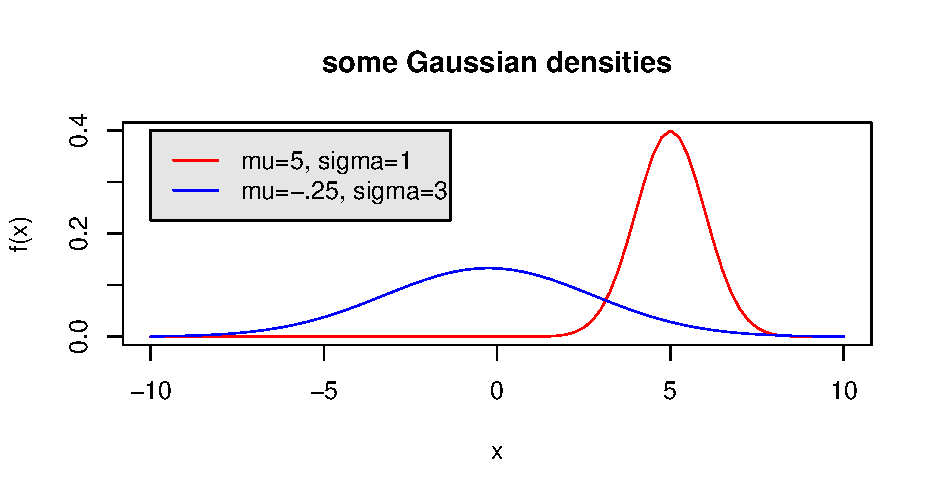
\includegraphics[width=100mm]{/home/taylor/UVa/all_teaching/3120_slides/4/4.3/pics/Rplot.pdf}
\end{center}

\end{frame}


%----------------------------------------------------------------------------------------


% \begin{frame}
% \frametitle{Proof}
% 
% Let's prove a standard normal $Z \sim \mathcal{N}(0,1)$ integrates to $1$. Or 
% \[
% \int_{-\infty}^{\infty}\frac{1}{\sqrt{2 \pi }} \exp\left[-\frac{z^2}{2} \right] dz = 1
% \]
% which is the same as 
% \[
% \int_{-\infty}^{\infty} \exp\left[-\frac{z^2}{2} \right] dz = \sqrt{2 \pi }
% \]
% or 
% \[
% \left( \int_{-\infty}^{\infty} \exp\left[-\frac{z^2}{2} \right] dz \right)^2 = 2 \pi
% \]
% 
% \end{frame}

%----------------------------------------------------------------------------------------


% \begin{frame}
% \frametitle{Proof}
% 
% Let $r = \sqrt{x^2 + y^2}$ and $\theta = \arctan|\frac{y}{x}|$. 
% 
% So $x = r \cos\theta$ and $y = r\sin\theta$ and 
% \begin{align*}
% \left( \int_{-\infty}^{\infty} \exp\left[-\frac{z^2}{2} \right] dz \right)^2 &= 
%     \left(\int_{-\infty}^{\infty} \exp\left[-\frac{x^2}{2} \right] dx\right) 
%     \left( \int_{-\infty}^{\infty} \exp\left[-\frac{y^2}{2} \right] dy \right)\\
% &= \int_{-\infty}^{\infty} \int_{-\infty}^{\infty} \exp\left[-\frac{x^2}{2} \right]
%     \exp\left[-\frac{y^2}{2} \right] dx dy \\
% &= \int_{-\infty}^{\infty} \int_{-\infty}^{\infty} \exp\left[-\frac{(x+y)^2}{2} \right]
%     dx dy \\
% \end{align*}
% 
% 
% 
% 
% \end{frame}

%----------------------------------------------------------------------------------------


\begin{frame}
\frametitle{Definition}

a special instance of the normal distribution is the \textbf{standard normal distribution}. You just set $\mu = 0$ and $\sigma^2 = 1$
\[
f(z;0,1) = \frac{1}{\sqrt{2 \pi }} \exp\left[-\frac{z^2}{2} \right] 
\]

where $-\infty < z < \infty$
\newline

shorthand: $Z \sim \mathcal{N}(0, 1)$
\newline

It's convention to use capital $Z$ when we're talking about standard normal rvs
\end{frame}

%----------------------------------------------------------------------------------------


\begin{frame}
\frametitle{Note}

When we're talking about probabilities, we can ``do algebra" inside the parentheses. E.g:
\[
P(a \le \mu + Z \sigma \le b) = P \left( \frac{a - \mu}{\sigma} \le Z \le \frac{b - \mu}{\sigma}\right)
\]
or
\[
P \left( \frac{1}{X} > - c \right) = P \left( X > \frac{1}{-c} \right)
\]
with $X,c > 0$ for the last one.
\end{frame}

%----------------------------------------------------------------------------------------

\begin{frame}
\frametitle{Notation}

A note on notation:
\newline

$z_{\alpha}$ denotes the $1-\alpha \times 100$th percentile for a standard normal distribution


\end{frame}

%----------------------------------------------------------------------------------------


\begin{frame}
\frametitle{Proposition}

We'll generalize this a bit later, but if
\[
X \sim \mathcal{N}(\mu, \sigma^2)
\]
then 
\[
aX + b \sim \mathcal{N}(a \mu + b, a^2 \sigma^2)
\]
That's why we go back and forth between $X = \mu + \sigma Z$ and $Z = \frac{X-\mu}{\sigma}$ a lot. They are both normal, but sometimes one will have more convenient parameters than the other. 

\end{frame}

%----------------------------------------------------------------------------------------


\begin{frame}
\frametitle{MGFs}

The normal mgf  for $\mathcal{N}(\mu, \sigma^2)$ is 
\[
M_X(t) = \exp\left[ \mu t + \sigma^2 t^2 / 2\right]
\]


\end{frame}

%----------------------------------------------------------------------------------------

\begin{frame}
\frametitle{MGFs}

Proof:
\begin{align*}
M_Z(t) &= E[e^{zt}] \\
&= \int e^{tz} \frac{1}{\sqrt{2\pi}} e^{-z^2/2}dz \\
&= \int \frac{1}{\sqrt{2\pi}} e^{-(z^2 - 2tz)/2}dz \\
&= \int \frac{1}{\sqrt{2\pi}} e^{-(z^2 - 2tz + t^2 - t^2)/2}dz \\
&= e^{t^2/2}  \int \frac{1}{\sqrt{2\pi}} e^{-(z^2 - 2tz + t^2 )/2}dz \\
&= e^{t^2/2}  \int \frac{1}{\sqrt{2\pi}} e^{-(z - t)^2/2}dz = e^{t^2/2}
\end{align*}

Then 
\[
M_X(t) = E[e^{t(\mu + Z \sigma)}] = e^{t\mu} E[e^{(t \sigma) Z}] = e^{t\mu} M_Z(t\sigma) = \exp\left[\mu t + \sigma^2t^2/2 \right]
\]
\end{frame}

%----------------------------------------------------------------------------------------

\begin{frame}
\frametitle{example}

Let $R$ denote a random yearly return on a financial asset. 

$R \sim \mathcal{N}(\mu, \sigma^2)$

We initially invest \$1. 

The value of our investment after a year is $I_1 = e^{R}$

What is the expected value of our investment after a year?


\end{frame}

%----------------------------------------------------------------------------------------
\begin{frame}
\frametitle{example}

We're looking for $E[e^{tR}]$, so we can plug in $t=1$. This particular MGF is:
\[
E[e^{tR}] = M_R(t) = \exp\left[\mu t + \sigma^2t^2/2 \right].
\]

where the last equality follows from two slides ago.
\newline

So instead of finding moments of $R$, or using it to find out what distribution transformations of $R$ follow, we can use MGFs for this too (in this literal way).
\newline

In chapter 5 we will go further and find the distribution of this random variable.
\end{frame}

%----------------------------------------------------------------------------------------

\end{document} 